\begin{figure}[H]
\centering
	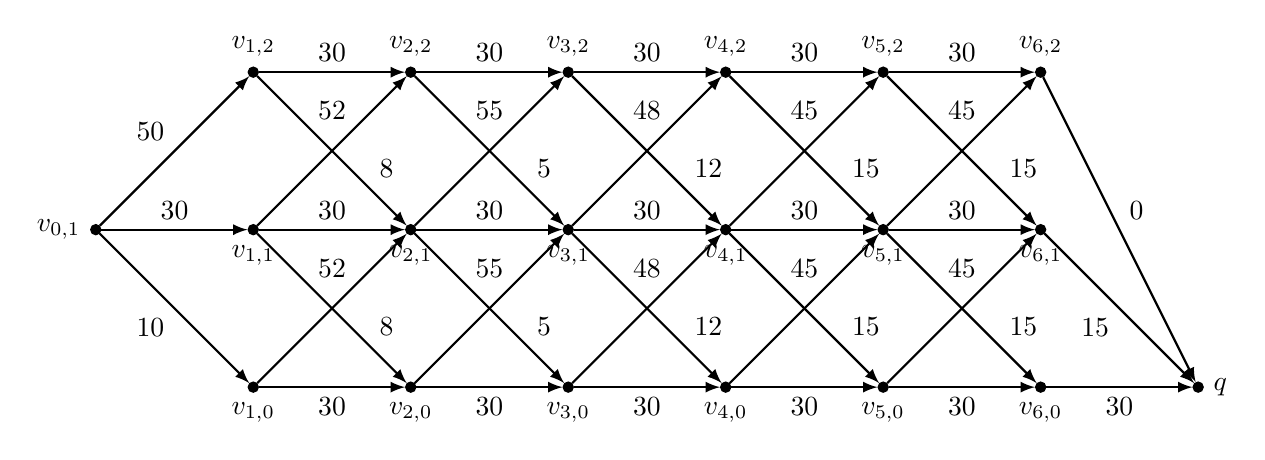
\begin{tikzpicture}

       \tikzset{enclosed/.style={draw, circle, inner sep=0pt, minimum size=.13cm, fill=black}}
%% Vertices
      	\node[enclosed, label={left: $v_{0,1}$}] (v1) at (0,2) {};
      	\node[enclosed, label={below: $v_{1,0}$}] (v2) at (2,0) {};
    		\node[enclosed, label={below: $v_{1,1}$}] (v3) at (2,2) {};
  	    \node[enclosed, label={above: $v_{1,2}$}] (v4) at (2,4) {};
     	\node[enclosed, label={below: $v_{2,0}$}] (v5) at (4,0) {};
     	\node[enclosed, label={below: $v_{2,1}$ }] (v6) at (4,2) {};
     	\node[enclosed, label={above: $v_{2,2}$}] (v7) at (4,4) {};
     	\node[enclosed, label={below:$v_{3,0}$ }] (v8) at (6,0) {};
     	\node[enclosed, label={below:$v_{3,1}$ }] (v9) at (6,2) {};
     	\node[enclosed, label={above:$v_{3,2}$ }] (v10) at (6,4) {};
     	\node[enclosed, label={below: $v_{4,0}$ }] (v11) at (8,0) {};
     	\node[enclosed, label={below:$v_{4,1}$ }] (v12) at (8,2) {};
      	\node[enclosed, label={above:$v_{4,2}$ }] (v13) at (8,4) {};
  	    \node[enclosed, label={below: $v_{5,0}$}] (v14) at (10,0) {};
  	    \node[enclosed, label={below:$v_{5,1}$ }] (v15) at (10,2) {};
     	\node[enclosed, label={above: $v_{5,2}$ }] (v16) at (10,4) {};
     	\node[enclosed, label={below:$v_{6,0}$ }] (v17) at (12,0) {};
     	 \node[enclosed, label={below:$v_{6,1}$}] (v18) at (12,2) {};
     	\node[enclosed, label={above: $v_{6,2}$}] (v19) at (12,4) {};
     	\node[enclosed, label={right: $q_{\slut}$ }] (v20) at (14,0) {};
     	
%Edges
		\path[->,>=latex,thick] (v1) edge node[midway, sloped, above, label={below: $10$ }] {} (v2);
		\path[->,>=latex,thick] (v1) edge node[midway, sloped, below, label={above: $30$ }] {} (v3);
		\path[->,>=latex,thick] (v1) edge node[midway, sloped, below, label={above: $50$ }] {} (v4);
		\path[->,>=latex,thick] (v2) edge node[midway, sloped, above, label={below: $30$ }] {} (v5);
		\path[->,>=latex,thick] (v2) edge node[midway, above, label={above: $52$ }] {} (v6);
		\path[->,>=latex,thick] (v3) edge node[near end, sloped, below, label={above: $8$ }] {} (v5);
		\path[->,>=latex,thick] (v3) edge node[midway, sloped, below, label={above: $30$ }] {} (v6);
		\path[->,>=latex,thick] (v3) edge node[midway, above, label={above: $52$ }] {} (v7);
		\path[->,>=latex,thick] (v4) edge node[near end, sloped, below, label={above: $8$ }] {} (v6);
		\path[->,>=latex,thick] (v4) edge node[midway, sloped, below, label={above: $30$ }] {} (v7);
		\path[->,>=latex,thick] (v5) edge node[midway, sloped, above, label={below: $30$ }] {} (v8);
		\path[->,>=latex,thick] (v5) edge node[midway, above, label={above: $55$ }] {} (v9);
		\path[->,>=latex,thick] (v6) edge node[near end, sloped, below, label={above: $5$ }] {} (v8);
		\path[->,>=latex,thick] (v6) edge node[midway, sloped, below, label={above: $30$ }] {} (v9);
		\path[->,>=latex,thick] (v6) edge node[midway, above, label={above: $55$ }] {} (v10);
		\path[->,>=latex,thick] (v7) edge node[near end, sloped, below, label={above: $5$ }] {} (v9);
		\path[->,>=latex,thick] (v7) edge node[midway, sloped, below, label={above: $30$ }] {} (v10);
		\path[->,>=latex,thick] (v8) edge node[midway, sloped, above, label={below: $30$ }] {} (v11);
		\path[->,>=latex,thick] (v8) edge node[midway, above, label={above: $48$ }] {} (v12);
		\path[->,>=latex,thick] (v9) edge node[near end, sloped, below, label={above: $12$ }] {} (v11);
		\path[->,>=latex,thick] (v9) edge node[midway, sloped, below, label={above: $30$ }] {} (v12);
		\path[->,>=latex,thick] (v9) edge node[midway, above, label={above: $48$ }] {} (v13);
		\path[->,>=latex,thick] (v10) edge node[near end, sloped, below, label={above: $12$ }] {} (v12);
		\path[->,>=latex,thick] (v10) edge node[midway, sloped, below, label={above: $30$ }] {} (v13);
		\path[->,>=latex,thick] (v11) edge node[midway, sloped, above, label={below: $30$ }] {} (v14);
		\path[->,>=latex,thick] (v11) edge node[midway, above, label={above: $45$ }] {} (v15);
		\path[->,>=latex,thick] (v12) edge node[near end, sloped, below, label={above: $15$ }] {} (v14);
		\path[->,>=latex,thick] (v12) edge node[midway, sloped, below, label={above: $30$ }] {} (v15);
		\path[->,>=latex,thick] (v12) edge node[midway, above, label={above: $45$ }] {} (v16);
		\path[->,>=latex,thick] (v13) edge node[near end, sloped, below, label={above: $15$ }] {} (v15);
		\path[->,>=latex,thick] (v13) edge node[midway, sloped, below, label={above: $30$ }] {} (v16);
		\path[->,>=latex,thick] (v14) edge node[midway, sloped, above, label={below: $30$ }] {} (v17);
		\path[->,>=latex,thick] (v14) edge node[midway, above, label={above: $45$ }] {} (v18);
		\path[->,>=latex,thick] (v15) edge node[near end, sloped, below, label={above: $15$ }] {} (v17);
		\path[->,>=latex,thick] (v15) edge node[midway, sloped, below, label={above: $30$ }] {} (v18);
		\path[->,>=latex,thick] (v15) edge node[midway, above, label={above: $45$ }] {} (v19);
		\path[->,>=latex,thick] (v16) edge node[near end, sloped, below, label={above: $15$ }] {} (v18);
		\path[->,>=latex,thick] (v16) edge node[midway, sloped, below, label={above: $30$ }] {} (v19);
		\path[->,>=latex,thick] (v17) edge node[midway, sloped, above, label={below: $30$ }] {} (v20);
		\path[->,>=latex,thick] (v18) edge node[midway, sloped, above, label={below: $15$ }] {} (v20);
		\path[->,>=latex,thick] (v19) edge node[midway, sloped, below, label={above: $0$ }] {} (v20);
	\end{tikzpicture}
	\caption{Forsimplet graf for gaslager ganget med -1 og med ikke-negative vægte.}
	\label{fig.gaslager_graf}
\end{figure}